% Read the readme first!
% options:
% - uulm-draft: show todonotes, links, linenumbers hide label names
% - uulm-draft-verbose: show todonotes, links, linenumbers, label names
% - uulm-release-electronic: show links, hide todonotes, linenumbers, label names
% - uulm-release-print hide everything
%

\documentclass[uulm-release-electronic]{thesis-uulm} % für die finale Abgabe
%\documentclass[uulm-draft]{thesis-uulm} % um ToDo's anzuzeigen

% workarround for some stupid error in combination with IEEEtran, bibtex and babel.
\makeatletter
\def\markboth#1#2{%
  \def\leftmark{\@IEEEcompsoconly{\sffamily}#1}%
  \def\rightmark{\@IEEEcompsoconly{\sffamily}#2}}
\makeatother

% Choose language
\usepackage[ngerman]{babel}
%% \usepackage[english]{babel}

\usepackage{float}

% Fonts
\renewcommand{\sfdefault}{phv}
\renewcommand{\rmdefault}{phv}
\renewcommand{\ttdefault}{pcr}

% Adjust variables
\author{Lukas Pellot}
\title{Projektionen in D3.js}
\email{lukas.pellot@uni-ulm.de}
\matnr{758179}	% Student ID

\type{Proseminararbeit} % Type of Thesis (Bachelors, Masters)
\jahr{Wintersemester 2017/18}

\gutachterA{Prof. Dr. Timo Ropinski} % First Reviewer
%\gutachterB{Prof. Dr. Un Leserlich}  % Second reviewer
\betreuer{Julian Kreiser} % supervisor

% Can be user to only compile parts of the document
\includeonly{
template/definitions,
chapters/introduction,
chapters/theory
}

% Definitions for code listings
%% definitions.tex
%%

%Listings für die Darstellung der Treiber im Anhang:
%-------------------------------------------------------
\usepackage{listings}

\usepackage{color}
\definecolor{gray}{rgb}{0.4,0.4,0.4}
\definecolor{darkblue}{rgb}{0.0,0.0,0.6}
\definecolor{cyan}{rgb}{0.0,0.6,0.6}

\lstset{
  basicstyle=\ttfamily,
  columns=fullflexible,
  showstringspaces=false,
  commentstyle=\color{gray}\upshape
}

\lstdefinelanguage{XML}
{
  morestring=[b]",
  morestring=[s]{>}{<},
  morecomment=[s]{<?}{?>},
  stringstyle=\color{black},
  identifierstyle=\color{darkblue},
  keywordstyle=\color{cyan},
  morekeywords={xmlns,version,type}% list your attributes here
}
%-----------------------------------------------------------


\begin{document}

\frontmatter %%%%%%%%%%%%%%%%%%%%%%%%%%%%%%%%%%%%%%%%%%%%%%%%%%%%%%%%%%%%%%%%%
\pagenumbering{roman}
\begin{nolinenumbers}
\maketitle

\copyrightpage % comment out if not wanted
\end{nolinenumbers}

\setstretch{1.2}

\begin{nolinenumbers}
\tableofcontents
\end{nolinenumbers}

\mainmatter %%%%%%%%%%%%%%%%%%%%%%%%%%%%%%%%%%%%%%%%%%%%%%%%%%%%%%%%%%%%%%%%%%
\pagenumbering{arabic}
%% introduction.tex
%%

\chapter{Einleitung}
\label{ch:introduction}

Seit jeher werden Landkarten genutzt, um die topologische Beschaffenheit der Welt sowie, vor allem in Zeiten der Globalisierung, (über-)regionale Sachverhalte und Statistiken grafisch aufbereitet darzustellen.

Allerdings bestehen zwei Problematiken. Dreidimensionale Strukturen wie Globen (und damit auch deren Oberflächen) können aufgrund des "Verlusts" einer Dimension grundsätzlich nur verzerrt auf zweidimensionalen Strukturen (wie Papier oder Computer-Bildschirmen) wiedergegeben werden. Außerdem gibt es unzählige Möglichkeiten, eine solche Verzerrung durchzuführen. Die Vereinheitlichung einer solchen Verzerrung (in Form einer Funktion) nennt man Projektion.

Die vorliegende Ausarbeitung beschäftigt sich mit solchen Projektionen. Es werden zunächst Projektionen im Allgemeinen und danach deren Implementierung und Nutzung in der JavaScript-Bibliothek D3.js erläutert.


%% basics.tex
%%
\chapter{Einführung in Projektionen}
\label{ch:theory}

\section{Allgemeines}

Will man einen Ausschnitt der Oberfläche einer Sphäre, beispielsweise ein Land auf dem Erdball, auf einer ebenen Oberfläche wie einem Bildschirm oder einem Blatt Papier darstellen, so muss eine Funktion aufgestellt werden, die einen dreidimensionalen Punkt (üblicherweise erfolgt die Darstellung hier durch ein Paar aus Breiten- und Längengrad) in einen zweidimensionalen Punkt umwandelt. Eine solche Funktion nennt man Projektion.

Hierbei ist zu beachten, dass mit dem Verlust einer räumlichen Dimension bei der Anwendung einer Projektion stets ein gewisser Informationsverlust beziehungsweise eine -verfälschung einhergeht. Betroffen sein können hierbei der Flächeninhalt der projizierten Struktur, die Länge einer Strecke innerhalb dieser, oder Winkel innerhalb eines Streckenverlaufs. Bewerkstelligt es eine Projektion, bei mehreren projizierten Strukturen eine der genannten Eigenschaften für alle Strukturen um einen konstanten Faktor verzerrt (üblicherweise verkleinert) wiederzugeben, wird diese Projektion flächen-/längen-/winkeltreu genannt.

\section{Kategorisierung von Projektionen}

Projektionen können in folgende Kategorien eingeteilt werden:

\paragraph{Azimutalprojektion}

Bei einer Azimutalprojektion wird die Sphäre ohne Zwischenschritte direkt auf eine Ebene projiziert.

\begin{figure}[H]
    \centering
    
    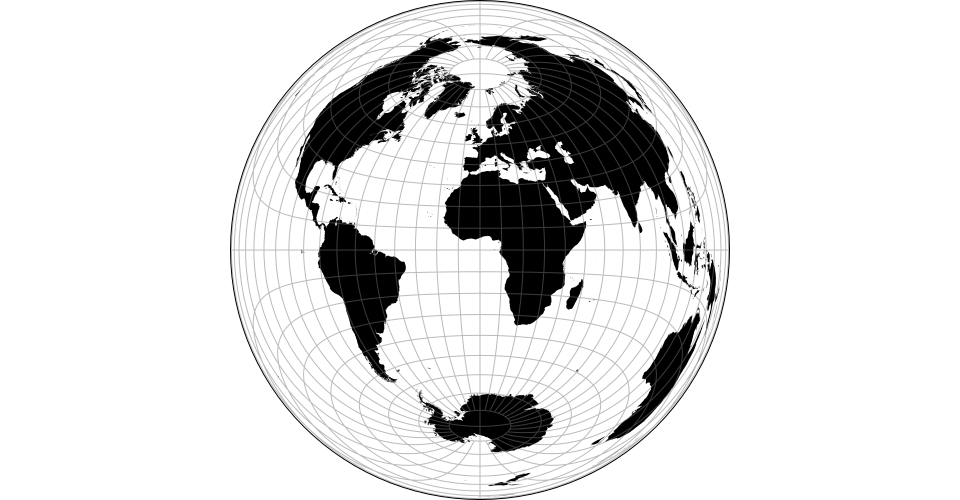
\includegraphics[width=.5\textwidth]{images/azimuthalEqualArea}
    \caption{Flächentreue Azimutalprojektion}
\end{figure}

\begin{figure}[H]
    \centering
    
    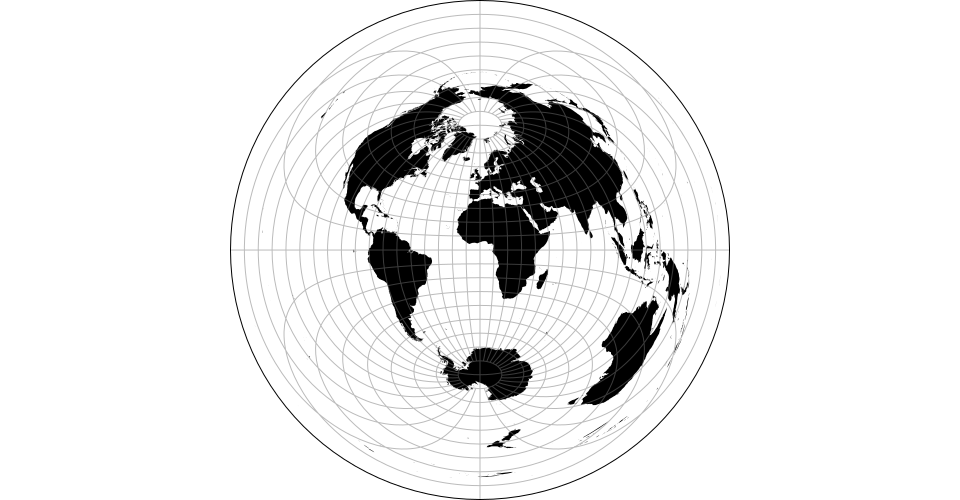
\includegraphics[width=.5\textwidth]{images/azimuthalEquidistant}
    \caption{Längentreue Azimutalprojektion}
\end{figure}

\paragraph{Konische Projektion}

Bei einer konischen Projektion wird die Sphäre zunächst auf einen Kegel projiziert. Dieser wird dann aufgeschnitten und auf eine Ebene ausgerollt.

\begin{figure}[H]
    \centering
    
    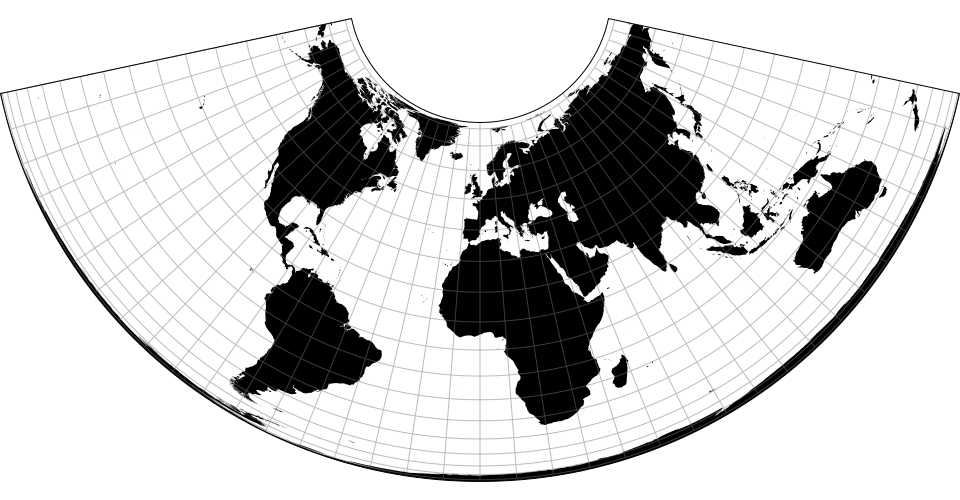
\includegraphics[width=.5\textwidth]{images/conicEqualArea}
    \caption{Flächentreue konische Projektion}
\end{figure}

\begin{figure}[H]
    \centering
    
    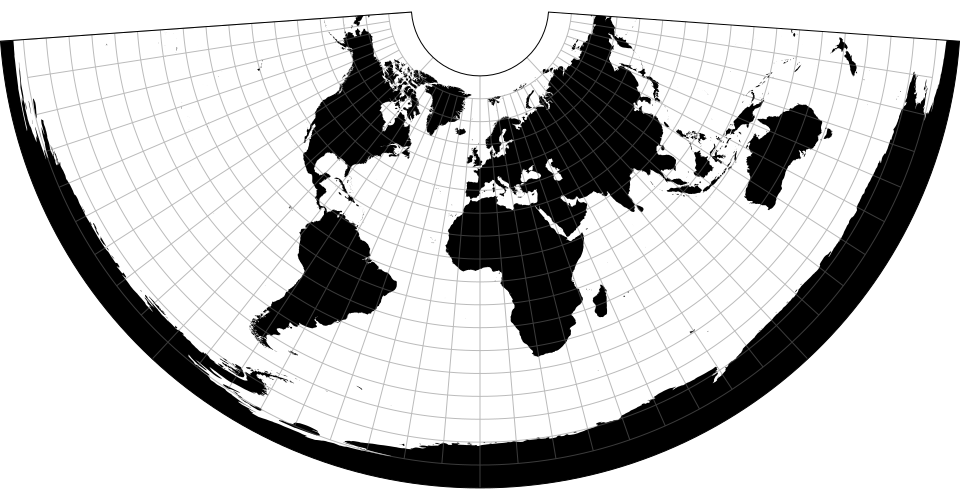
\includegraphics[width=.5\textwidth]{images/conicEquidistant}
    \caption{Längentreue konische Projektion}
\end{figure}

\paragraph{Zylindrische Projektion}

Bei einer zylindrischen Projektion wird die Sphäre zunächst auf einen Zylinder projiziert. Dieser wird dann aufgeschnitten und auf eine Ebene ausgerollt.

\begin{figure}[H]
    \centering
    
    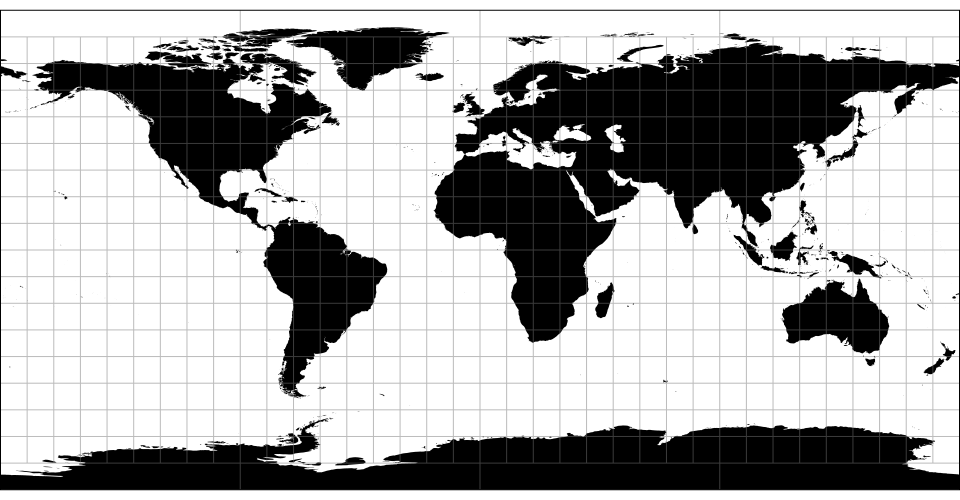
\includegraphics[width=.5\textwidth]{images/equirectangular}
    \caption{Längentreue Zylinderprojektion}
\end{figure}

\begin{figure}[H]
    \centering
    
    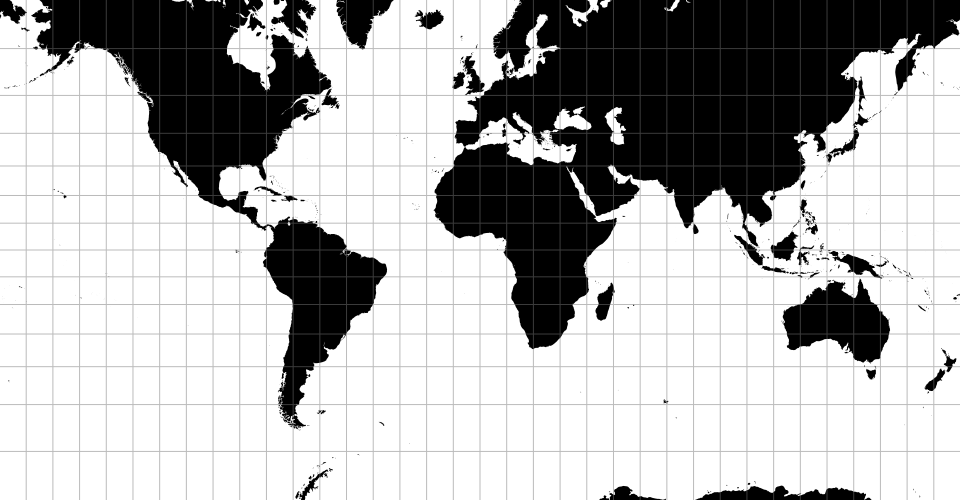
\includegraphics[width=.5\textwidth]{images/mercator}
    \caption{Winkeltreue Zylinderprojektion}
\end{figure}

\paragraph{Pseudozylindrische Projektion}

Pseudozylindrische Projektionen stellen eine Verallgemeinerung zylindrischer Projektionen dar. Breitengrade werden ebenso als parallele Linien projiziert, allerdings sind Höhengrade der konkreten Projektion entsprechend geneigt.

\begin{figure}[H]
    \centering
    
    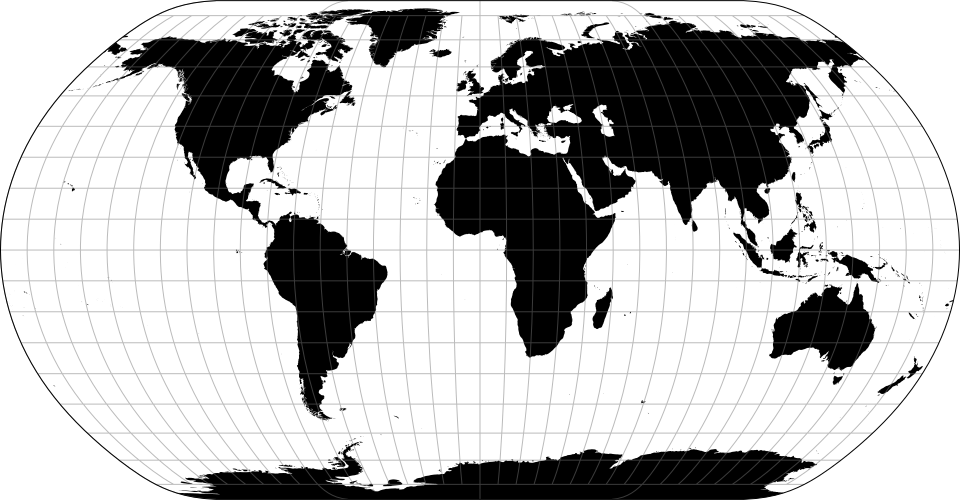
\includegraphics[width=.5\textwidth]{images/naturalEarth1}
    \caption{\glqq Natural Earth\grqq -Projektion}
\end{figure}

\paragraph{Zusammengesetzte Projektion}

Zusammengesetzte Projektionen kombinieren verschiedene der oben genannten Projektionen. Im Gegensatz zu den anderen Kategorien werden zusammengesetzte Projektionen selten für die Darstellung der gesamten Welt, sondern häufiger lediglich für Ausschnitte ebendieser genutzt.

\begin{figure}[H]
    \centering
    
    \includegraphics[width=.5\textwidth]{images/albersUSA}
    \caption{Albers-USA-Projektion}
\end{figure}

Hier wird die Albers-USA-Projektion gezeigt, die den Hauptteil der USA als konische Projektion, allerdings aus Platzgründen Alaska und Hawaii in der linken unteren Ecke um einen Faktor von etwa $0.35$ verkleinert als zylindrische Projektion darstellt.

\paragraph{Anmerkung}

Bei Betrachtung der Abbildungen fällt auf, dass keine der Kategorien Treue hinsichtlich einer Eigenschaft bedingt oder fördert, und diese lediglich der Optik dienlich sind.

\include{chapters/projections-in-d3}

\backmatter %%%%%%%%%%%%%%%%%%%%%%%%%%%%%%%%%%%%%%%%%%%%%%%%%%%%%%%%%%%%%%%%%%

%\bibliographystyle{natdin}
\bibliographystyle{IEEEtranS}	% alternativer Stil
\bibliography{bibliography} % Bib-Datei

\end{document}
